\documentclass[12pt,a4paper]{article}
\usepackage[utf8]{inputenc}
\usepackage[english]{babel}
\usepackage{geometry}
\usepackage{graphicx}
\usepackage{float}
\usepackage{placeins}
\usepackage{caption}
\usepackage{hyperref}
\usepackage{enumitem}
\usepackage{fancyhdr}
\usepackage{svg}
\usepackage{titlesec}
\usepackage{tocloft}
\usepackage{amsmath}
\usepackage{amsfonts}
\usepackage{amssymb}
\usepackage{textcomp} % or amssymb

% Page setup
\geometry{margin=1in}
\pagestyle{fancy}
\fancyhf{}
\fancyhead[L]{ENSIASD E-Learning Platform}
\fancyhead[R]{\thepage}
\renewcommand{\headrulewidth}{0.4pt}

% Title formatting
\titleformat{\section}{\Large\bfseries}{\thesection}{1em}{}
\titleformat{\subsection}{\large\bfseries}{\thesubsection}{1em}{}
\titleformat{\subsubsection}{\normalsize\bfseries}{\thesubsubsection}{1em}{}

% Hyperlink setup
\hypersetup{
    colorlinks=true,
    linkcolor=blue,
    filecolor=magenta,      
    urlcolor=cyan,
    pdftitle={ENSIASD E-Learning Platform Report},
    pdfauthor={ENSIASD Taroudant},
}

\begin{document}

% Title Page
\begin{titlepage}
% \BgThispage % Assuming \BgThispage is a custom command for a background image; ensure it's defined or remove if not used.

  \begin{center}
    \vspace*{-3cm} % Pulls the logo up to the very top
    
\includegraphics[width=1\textwidth]{images/logo.png}\\[0.1cm]
    \vspace*{0.2cm} % Space after logo
  \end{center}

  \begin{center}
    {\Large \emph{Formation:}}\\[0.2cm] % Reduced spacing
    {\large Software Engineering} \\[0.7cm] % Reduced spacing

    % Enhanced project report title with reduced spacing
    \begin{center}
      \colorbox{white!90}{\parbox{0.8\textwidth}{
        \centering
        \vspace{0.2cm} % Reduced padding
        {\Large\bfseries RAPPORT DE PROJET}\\[0.1cm] % Reduced spacing
        {\large\textit{Module: Technologies Web}}
        \vspace{0.2cm} % Reduced padding
      }}
    \end{center}
    \vspace{0.5cm} % Reduced spacing

    % Title with reduced spacing
    \rule{\linewidth}{0.5mm} \\[0.1cm]
    {\huge \bfseries Development of an E-Learning Platform for ENSIASD \\[0.1cm]}
    \rule{\linewidth}{0.5mm} \\[1cm] % Reduced spacing
    
    \begin{center}
      \includesvg[width=0.10\textwidth]{images/laravel.svg} \hspace{1cm}
      \includesvg[width=0.10\textwidth]{images/react_light.svg} \hspace{1cm}
      \includesvg[width=0.10\textwidth]{images/mysql.svg} \hspace{1cm}
      \includesvg[width=0.15\textwidth]{images/tailwindcss.svg} % Reduced size
    \end{center}

    % Authors and supervisor side by side with reduced spacing
    \vspace{6cm} % Reduced spacing

    \begin{minipage}[t]{0.45\textwidth}
      \begin{flushleft}
        {\Large \emph{Réalisé par:}}\\[0.2cm] % Reduced spacing
        {\large 
          MOHAMED EL GUARIR \\[0.1cm] % Reduced spacing
          MOHAMED EL HADDATI \\[0.1cm] % Reduced spacing
          DOUNYA ZAHIDI \\[0.1cm] % Reduced spacing
          BAHRI MALAK \\[0.1cm] % Reduced spacing
        }
      \end{flushleft}
    \end{minipage}
    \hfill
    \begin{minipage}[t]{0.45\textwidth}
      \begin{flushright}
        {\Large \emph{Supervised by:}}\\[0.2cm] % Reduced spacing
        {\large 
          M. Mohamed Saad AZIZI \\[0.1cm] % Reduced spacing
        }
      \end{flushright}
    \end{minipage}

    \vspace*{3cm} % Push to bottom of page with minimal space
    % Bottom of the page (moved closer to bottom)
    {\large Année universitaire: 2024-2025}
  \end{center}
\end{titlepage}

% Table of Contents
\tableofcontents
\newpage
\listoffigures

\section{Introduction}

The ENSIASD E-Learning Platform represents a comprehensive digital educational solution tailored specifically for ENSIASD Taroudant, a prominent higher education institution. This report presents a detailed examination of the platform's architecture, functionality, and technical implementation, drawing from extensive analysis of the existing codebase, database structure, and system configuration.

ENSIASD Taroudant's E-Learning Platform emerges from the institution's commitment to educational innovation and digital transformation. At its core, the platform facilitates meaningful connections between instructors and students through technology, creating an environment where educational content delivery, student engagement, and administrative oversight converge seamlessly. The system recognizes that effective e-learning requires more than content delivery—it demands interaction, feedback, and community.

The platform serves three distinct user communities within ENSIASD Taroudant: students seeking flexible access to quality education, instructors requiring comprehensive tools for course delivery and student engagement, and administrators managing institutional content and system oversight.

This documentation encompasses both the technical foundations that power the platform and the user-centric features that define the learning experience. The analysis reveals a well-structured system that balances complexity with usability, offering robust functionality while maintaining the flexibility necessary for diverse educational scenarios. This report serves educators, administrators, and technical stakeholders who seek to understand the platform's capabilities and potential for enhancing the educational experience at ENSIASD Taroudant.

\subsection{Core Platform Capabilities}

\begin{itemize}
    \item \textbf{Dynamic Course Environment:} Instructors create rich, multi-layered courses featuring diverse content types, from traditional text and file resources to interactive quizzes and external learning materials.
    \item \textbf{Comprehensive Assessment Tools:} The platform supports varied assessment methods including assignments with flexible submission options, interactive quizzes, and detailed grading workflows with instructor feedback.
    \item \textbf{Collaborative Learning Spaces:} Course-specific discussion forums and announcement systems foster communication between instructors and students, creating virtual learning communities.
    \item \textbf{Institutional Web Presence:} A professionally designed public website showcases ENSIASD Taroudant's programs, mission, and educational offerings while providing prospective students with essential information.
    \item \textbf{Role-Based Access Management:} The platform implements sophisticated user role systems ensuring appropriate access levels:
    \begin{itemize}
        \item \textbf{Students:} Access course materials, submit assignments, participate in discussions, and track academic progress.
        \item \textbf{Instructors:} Design courses, manage content, assess student work, and facilitate learning experiences.
        \item \textbf{Administrators:} Oversee institutional content, manage public website elements, and maintain system-wide functionality.
    \end{itemize}
\end{itemize}

\section{User Roles and Functionality}
\label{sec:user-roles-functionality}

The platform's effectiveness stems from its careful attention to the distinct needs of each user type within the educational ecosystem. Rather than adopting a one-size-fits-all approach, the system provides tailored experiences that enhance productivity and engagement for students, instructors, and administrators alike.

\subsection{User Roles}

The platform defines three primary user roles, each with specific capabilities:

\begin{itemize}
    \item \textbf{Student:}
    \begin{itemize}
        \item \textbf{Course Interaction:} Enrolls in available courses using course codes or invite links. Accesses all published course materials, including chapters, uploaded resources (documents, videos, links), and embedded rich text content.
        \item \textbf{Assignments \& Quizzes:} Submits assignments as per instructor requirements (potentially including text and file uploads). Takes quizzes designed to assess understanding of course content.
        \item \textbf{Communication:} Participates in course-specific discussion forums by creating new threads or commenting on existing ones. Views course announcements made by instructors and can comment on them.
        \item \textbf{Progress & Profile:} Tracks their progress and grades for assignments and quizzes (implied by submission and grading features). Manages their personal profile information (name, avatar, etc.).
    \end{itemize}
    \item \textbf{Instructor:}
    \begin{itemize}
        \item \textbf{Course Management:} Creates new courses, providing details such as title, description, image, category, and a unique color theme. Organizes courses into reorderable chapters. Adds and manages diverse learning resources within chapters (rich text, file attachments, external web links). Controls course status (draft, published, archived).
        \item \textbf{Assessment Management:} Creates, edits, and manages assignments with detailed instructions, due dates, and optional attachments. Develops and administers quizzes with various question types and options.
        \item \textbf{Student Interaction \& Grading:} Views student submissions for assignments. Provides grades and textual feedback on submissions.
        \item \textbf{Communication \& Engagement:} Posts course-specific announcements to students, which can include content and attachments. Manages and participates in course discussion forums.
        \item \textbf{Enrollment Management:} Manages student enrollments within their courses, including the ability to remove students if necessary.
        \item \textbf{Dashboard \& Analytics:} Accesses a dedicated dashboard providing statistics on their courses, such as total student numbers, active student counts, enrollment trends over time, and distribution of resource types used.
        \item \textbf{Profile Management:} Manages their personal and professional profile information.
    \end{itemize}
    \item \textbf{Administrator:}
    \begin{itemize}
        \item \textbf{Public Website Content Management:} Manages the content of the public-facing website pages, including the Home page (e.g., hero section text, images, links), About page (mission, vision, features, stats), Contact page (contact details, map), and Publications/Announcements page. This is managed through a dedicated interface in the backend.
    \end{itemize}
\end{itemize}

\subsection{Platform Features}

Beyond role-specific capabilities, the platform integrates numerous features that work together to create a cohesive educational environment. These features address the fundamental requirements of modern e-learning while providing flexibility for diverse teaching and learning styles:

\begin{itemize}
    \item \textbf{User Authentication \& Authorization:}
    \begin{itemize}
        \item Secure user registration and login mechanisms.
        \item Password management (e.g., reset functionality).
        \item Role-based access control, ensuring users only access features relevant to their role.
        \item A profile completion step for new users to ensure necessary information is provided.
    \end{itemize}
    \item \textbf{Course Creation \& Management:}
    \begin{itemize}
        \item Instructors can create courses with comprehensive details: title, description, cover image, category, display color, and status (draft, published, archived).
        \item Automatic generation of unique course codes and shareable invite tokens for easy student enrollment.
        \item Courses can be structured into logical chapters, which instructors can reorder as needed.
        \item A variety of resource types can be added to chapters:
        \begin{itemize}
            \item \textbf{Rich Text:} For creating formatted textual content directly on the platform.
            \item \textbf{Attachments:} For uploading files (documents, presentations, media).
            \item \textbf{External Links:} For linking to external web resources.
        \end{itemize}
    \end{itemize}
    \item \textbf{Assignment Management:}
    \begin{itemize}
        \item Instructors can create assignments with titles, detailed instructions, specific due dates, and attach relevant files.
        \item Control over assignment visibility through a publish/unpublish mechanism.
    \end{itemize}
    \item \textbf{Submission System:}
    \begin{itemize}
        \item Students can submit their work for assignments, typically involving text input and/or file uploads.
        \item Instructors have an interface to view all submissions for an assignment, access submitted files, and assign grades and provide written feedback.
    \end{itemize}
    \item \textbf{Quiz System:}
    \begin{itemize}
        \item Includes functionality for generating quizzes (\texttt{QuizController::generateQuiz}).
        \item Supports the creation of quiz questions, multiple-choice options (or other question types), and tracks student answers. This allows for automated or instructor-led assessment of learning.
    \end{itemize}
    \item \textbf{Announcement System:}
    \begin{itemize}
        \item Instructors can create and post announcements visible to all students within a specific course.
        \item Announcements can contain formatted text and include file attachments.
        \item A commenting feature allows for interaction and clarification on announcements.
    \end{itemize}
    \item \textbf{Discussion Forum:}
    \begin{itemize}
        \item Each course has its own dedicated discussion forum.
        \item Students and instructors can create new discussion threads on relevant topics.
        \item Users can post comments within threads, fostering a collaborative learning environment.
    \end{itemize}
    \item \textbf{Instructor Dashboard:}
    \begin{itemize}
        \item A personalized dashboard for instructors provides key statistics and insights into their courses and student engagement. This includes:
        \begin{itemize}
            \item Aggregate counts: total students, number of courses.
            \item Activity metrics: currently active students.
            \item Growth indicators: percentage changes in student numbers and course creation.
            \item Visualizations: Charts displaying enrollment trends over time and a breakdown of resource types used across courses.
        \end{itemize}
    \end{itemize}
    \item \textbf{Public Website \& Content Management:}
    \begin{itemize}
        \item The platform includes a public-facing website with several key pages:
        \begin{itemize}
            \item \textbf{Home:} Landing page with introductory content, featured courses, and platform highlights.
            \item \textbf{About:} Information about ENSIASD Taroudant and the e-learning platform's mission and features.
            \item \textbf{Courses:} A public listing of available courses, potentially with search and filtering capabilities by category.
            \item \textbf{Publications:} A section for general announcements, news, or articles from the institution.
            \item \textbf{Contact:} Contact information and a contact form or map.
        \end{itemize}
        \item The content for these public pages is dynamically manageable by an Administrator via a backend interface, allowing updates to text, images, and other elements without code changes.
    \end{itemize}
    \item \textbf{Profile Management:}
    \begin{itemize}
        \item All users (Students, Instructors, Administrators) can manage their personal profile information, including name, email, password, and avatar.
    \end{itemize}
\end{itemize}
\clearpage



\section{System Architecture Overview}
This diagram presents the platform's technical architecture, illustrating how different software layers interact to deliver the complete user experience:
\begin{figure}[H] % Using [H] to suggest placing it "here". Adjust if needed.
    \centering       
    \includegraphics[width=0.8\textwidth,height=0.85\textheight,keepaspectratio]{system-architecture-overview.png}
    \caption{System Architecture flowchart}
    \label{fig:system-architecture-overview}
\end{figure}
\FloatBarrier % Ensure figure is placed before continuing

\begin{itemize}
    \item \textbf{Components:}
    \begin{itemize}
        \item \textbf{Client Tier:}
        \begin{itemize}
            \item \textbf{Web Browser:} Renders the UI (React components via Inertia.js), handles user input, executes client-side JavaScript.
        \end{itemize}
        \item \textbf{Application Tier:}
        \begin{itemize}
            \item \textbf{Web Server (e.g., Nginx, Apache):} Receives HTTP requests, serves static assets, acts as a reverse proxy for the application.
            \item \textbf{Laravel Application (PHP-FPM):}
            \begin{itemize}
                \item \textbf{Routing Engine:} Maps URLs to controller actions.
                \item \textbf{Controllers:} Handle HTTP requests, interact with models and services, prepare data for views/Inertia responses.
                \item \textbf{Models (Eloquent ORM):} Represent database tables, manage data persistence and relationships.
                \item \textbf{Middleware:} Handles cross-cutting concerns (authentication, CSRF, Inertia requests).
                \item \textbf{Inertia.js Adapter:} Bridges Laravel backend with React frontend.
                \item \textbf{Services:} Encapsulate specific business logic (e.g., QuizService, NotificationService - if explicitly created).
            \end{itemize}
        \end{itemize}
        \item \textbf{Data Tier:}
        \begin{itemize}
            \item \textbf{Database Server (e.g., MySQL, PostgreSQL, SQLite):} Stores all persistent application data (users, courses, submissions, etc.).
            \item \textbf{Cache Server (e.g., Redis):} Stores session data, cached queries, etc.
        \end{itemize}
        \item \textbf{External Services / Storage:}
        \begin{itemize}
            \item \textbf{File Storage (AWS S3):} Stores user-uploaded files (avatars, course materials, assignment attachments).
            \item \textbf{Email Service:} For sending transactional emails (verification, notifications).
        \end{itemize}
    \end{itemize}
    \item \textbf{Key Interactions:}
    \begin{itemize}
        \item Browser \texttt{<->} Web Server (HTTP/HTTPS)
        \item Web Server \texttt{<->} Laravel Application (FastCGI/PHP-FPM)
        \item Laravel Application \texttt{<->} Database Server (SQL)
        \item Laravel Application \texttt{<->} Cache Server
        \item Laravel Application \texttt{<->} File Storage
    \end{itemize}
\end{itemize}
\clearpage


\section{Technologies and Tools Used}
\label{sec:technologies-tools}

The platform's technical foundation reflects careful consideration of performance, maintainability, and developer experience. Each technology choice contributes to a cohesive development environment that supports rapid iteration while ensuring production reliability:

\subsection{Backend}
\begin{itemize}
    \item \textbf{Programming Language:} PHP (Version 8.3+)
    \item \textbf{Framework:} Laravel (Version 12)
    \item \textbf{Key PHP Libraries \& Packages:}
    \begin{itemize}
        \item \texttt{inertiajs/inertia-laravel}: Server-side adapter for Inertia.js, facilitating integration with the React frontend.
        \item \texttt{prism-php/prism}: Laravel package for integrating Large Language Models (LLMs).
        \item \texttt{tightenco/ziggy}: Enables the use of Laravel named routes within JavaScript.
        \item \texttt{league/flysystem-aws-s3-v3}: Provides an abstraction for file storage, configured for AWS S3. (Also supports local and other drivers).
        \item \texttt{predis/predis}: A flexible and feature-complete Redis client for PHP.
    \end{itemize}
\end{itemize}

\subsection{Frontend}
\begin{itemize}
    \item \textbf{Programming Languages:} TypeScript, JavaScript (ES6+)
    \item \textbf{Framework/Library:} React (Version 19)
    \item \textbf{SPA Integration:} Inertia.js (using \texttt{@inertiajs/react} adapter) for building a modern, single-page application experience with server-driven routing.
    \item \textbf{Key JavaScript Libraries \& Packages:}
    \begin{itemize}
        \item \textbf{UI \& Components:}
        \begin{itemize}
            \item \texttt{@radix-ui/*}: A comprehensive suite of unstyled, accessible UI primitives (e.g., Dialog, Dropdown, Select, Tooltip) used as the foundation for custom components (likely following a Shadcn UI-like pattern).
            \item \texttt{lucide-react}: For a wide range of SVG icons.
            \item \texttt{@headlessui/react}: Unstyled, fully accessible UI components.
            \item \texttt{cmdk}: Command menu component for quick navigation and actions.
            \item \texttt{embla-carousel-react}: A bare-bones carousel library.
            \item \texttt{sonner}: For displaying toast notifications.
            \item \texttt{recharts}: A composable charting library.
            \item \texttt{react-day-picker}: Date picker component.
            \item \texttt{vaul}: Drawer component.
        \end{itemize}
        \item \textbf{Text Editing:}
        \begin{itemize}
            \item \texttt{@tiptap/react} \& extensions: A headless, framework-agnostic rich text editor.
        \end{itemize}
        \item \textbf{Drag \& Drop:}
        \begin{itemize}
            \item \texttt{@dnd-kit/core} \& \texttt{@dnd-kit/sortable}: For implementing drag and drop interfaces.
        \end{itemize}
        \item \textbf{Forms \& Validation:}
        \begin{itemize}
            \item \texttt{zod} \& \texttt{zod-form-data}: For robust schema definition and validation.
            \item \texttt{react-dropzone}: For handling file uploads via drag and drop.
            \item \texttt{input-otp}: One-time password input component.
        \end{itemize}
        \item \textbf{Tables:}
        \begin{itemize}
            \item \texttt{@tanstack/react-table}: Headless UI for building powerful tables and datagrids.
        \end{itemize}
        \item \textbf{Animation:}
        \begin{itemize}
            \item \texttt{framer-motion}: A production-ready motion library for React.
        \end{itemize}
        \item \textbf{Utilities:}
        \begin{itemize}
            \item \texttt{date-fns}: Modern JavaScript date utility library.
            \item \texttt{next-themes}: For theme management (e.g., light/dark mode).
        \end{itemize}
    \end{itemize}
\end{itemize}

\subsection{Database}
\begin{itemize}
    \item \textbf{Development Default:} SQLite
    \item \textbf{Production Options:} MySQL, MariaDB, PostgreSQL, SQL Server (as per Laravel's standard support and \texttt{config/database.php}).
    \item \textbf{Caching / Key-Value Store:} Redis (client \texttt{predis/predis} configured).
\end{itemize}

\subsection{Styling}
\begin{itemize}
    \item \textbf{CSS Framework:} Tailwind CSS (Version 4)
    \item \textbf{Utility Libraries:}
    \begin{itemize}
        \item \texttt{class-variance-authority} (CVA): For creating type-safe, reusable UI components with variants.
        \item \texttt{clsx}: A tiny utility for constructing \texttt{className} strings conditionally.
        \item \texttt{tailwind-merge}: Utility to merge Tailwind CSS classes without style conflicts.
        \item \texttt{tailwindcss-animate}: Plugin for Tailwind CSS that adds enter/exit animations.
        \item \texttt{@tailwindcss/typography}: Tailwind CSS plugin for styling prose/HTML content.
    \end{itemize}
\end{itemize}

\subsection{Build \& Development Tools}
\begin{itemize}
    \item \textbf{JavaScript Bundler \& Dev Server:} Vite
    \item \textbf{PHP Dependency Manager:} Composer
    \item \textbf{JavaScript Package Manager:} npm (inferred from \texttt{package-lock.json}, though \texttt{bun.lock} also exists, indicating Bun might be used by some developers or in CI).
    \item \textbf{Version Control:} Git
    \item \textbf{Local Development Environment:} Laravel Sail (Docker-based, provides a standardized local development experience).
    \item \textbf{Debugging (Backend):} \texttt{barryvdh/laravel-debugbar} for in-browser debugging information.
    \item \textbf{Linters \& Formatters:}
    \begin{itemize}
        \item ESLint (JavaScript/TypeScript linter)
        \item Prettier (Code formatter)
        \item Laravel Pint (PHP code style fixer)
    \end{itemize}
\end{itemize}

\subsection{Server Environment}
\begin{itemize}
    \item \textbf{Web Server:} Nginx or Apache
    \item \textbf{PHP Runtime:} PHP-FPM (FastCGI Process Manager)
    \item \textbf{Database Server:} (MySQL Server)
    \item \textbf{Node.js:} Required for the frontend build process.
\end{itemize}
% \clearpage




\section{Database Architecture and Data Modeling}
\label{sec:database-architecture}

The platform's data architecture reflects the complex relationships inherent in educational environments. The database design accommodates diverse content types, user interactions, and assessment methods while maintaining referential integrity and supporting efficient queries. The following entities form the foundation of the platform's data model:

\subsection{Core Database Entities}

\begin{itemize}
    \item \textbf{User (\texttt{users} table):}
    \begin{itemize}
        \item \textbf{Attributes:} \texttt{id} (PK), \texttt{name}, \texttt{username}, \texttt{email} (unique), \texttt{avatar}, \texttt{role} (e.g., student, instructor, admin), \texttt{profile\_completed\_at} (timestamp), \texttt{password}, \texttt{email\_verified\_at} (timestamp), \texttt{remember\_token}, \texttt{created\_at}, \texttt{updated\_at}.
        \item \textbf{Relationships:}
        \begin{itemize}
            \item \texttt{InstructorProfile}: One-to-One (User has one InstructorProfile). Foreign Key: \texttt{instructor\_profiles.user\_id}.
            \item \texttt{CourseEnrollment}: One-to-Many (User has many CourseEnrollments). Foreign Key: \texttt{course\_enrollments.user\_id}.
            \item \texttt{Course} (as instructor): One-to-Many (User (instructor) has many Courses). Foreign Key: \texttt{courses.instructor\_id}.
            \item \texttt{CourseThread} (as author): One-to-Many (User has many CourseThreads). Foreign Key: \texttt{course\_threads.author\_id}.
            \item \texttt{ThreadComment} (as author): One-to-Many (User has many ThreadComments). Foreign Key: \texttt{thread\_comments.author\_id}.
            \item \texttt{Submission}: One-to-Many (User has many Submissions). Foreign Key: \texttt{submissions.user\_id}.
            \item \texttt{Announcement} (as author): One-to-Many (User has many Announcements). Foreign Key: \texttt{announcements.user\_id}.
            \item \texttt{AnnouncementComment} (as author): One-to-Many (User has many AnnouncementComments). Foreign Key: \texttt{announcement\_comments.user\_id}.
            \item \texttt{courses} (as student): Many-to-Many via \texttt{CourseEnrollment} (User belongs to many Courses).
        \end{itemize}
    \end{itemize}
    \item \textbf{InstructorProfile (\texttt{instructor\_profiles} table):}
    \begin{itemize}
        \item \textbf{Attributes:} \texttt{id} (PK), \texttt{user\_id} (FK to \texttt{users.id}), \texttt{bio}, \texttt{expertise\_areas} (array/JSON), \texttt{social\_links} (array/JSON), \texttt{created\_at}, \texttt{updated\_at}.
        \item \textbf{Relationships:}
        \begin{itemize}
            \item \texttt{User}: One-to-One (InstructorProfile belongs to one User).
        \end{itemize}
    \end{itemize}
    \item \textbf{Course (\texttt{courses} table):}
    \begin{itemize}
        \item \textbf{Attributes:} \texttt{id} (PK), \texttt{instructor\_id} (FK to \texttt{users.id}), \texttt{title}, \texttt{description}, \texttt{image} (path/URL), \texttt{code} (unique course code), \texttt{invite\_token} (unique for link-based enrollment), \texttt{color}, \texttt{category}, \texttt{status} (enum: draft, published, archived), \texttt{published\_at} (timestamp), \texttt{created\_at}, \texttt{updated\_at}.
        \item \textbf{Relationships:}
        \begin{itemize}
            \item \texttt{User} (instructor): Many-to-One (Course belongs to one User (instructor)).
            \item \texttt{Chapter}: One-to-Many (Course has many Chapters). Foreign Key: \texttt{chapters.course\_id}.
            \item \texttt{CourseEnrollment}: One-to-Many (Course has many CourseEnrollments). Foreign Key: \texttt{course\_enrollments.course\_id}.
            \item \texttt{CourseThread}: One-to-Many (Course has many CourseThreads). Foreign Key: \texttt{course\_threads.course\_id}.
            \item \texttt{Announcement}: One-to-Many (Course has many Announcements). Foreign Key: \texttt{announcements.course\_id}.
            \item \texttt{Assignment}: One-to-Many (Course has many Assignments). Foreign Key: \texttt{assignments.course\_id}.
            \item \texttt{students} (Users): Many-to-Many via \texttt{CourseEnrollment} (Course has many Students).
        \end{itemize}
    \end{itemize}
    \item \textbf{Chapter (\texttt{chapters} table):}
    \begin{itemize}
        \item \textbf{Attributes:} \texttt{id} (PK), \texttt{course\_id} (FK to \texttt{courses.id}), \texttt{title}, \texttt{description}, \texttt{position} (integer for ordering), \texttt{created\_at}, \texttt{updated\_at}.
        \item \textbf{Relationships:}
        \begin{itemize}
            \item \texttt{Course}: Many-to-One (Chapter belongs to one Course).
            \item \texttt{Resource}: One-to-Many (Chapter has many Resources). Foreign Key: \texttt{resources.chapter\_id}.
        \end{itemize}
    \end{itemize}
    \item \textbf{Resource (\texttt{resources} table):} (Central table for typed resources)
    \begin{itemize}
        \item \textbf{Attributes:} \texttt{id} (PK), \texttt{chapter\_id} (FK to \texttt{chapters.id}), \texttt{title}, \texttt{resource\_type} (enum: 'rich\_text', 'attachment\_collection', 'external\_link', 'quiz'), \texttt{position} (integer for ordering), \texttt{metadata} (JSON), \texttt{created\_at}, \texttt{updated\_at}.
        \item \textbf{Relationships:}
        \begin{itemize}
            \item \texttt{Chapter}: Many-to-One (Resource belongs to one Chapter).
            \item \texttt{RichTextResource}: One-to-One. Foreign Key: \texttt{rich\_text\_resources.resource\_id}.
            \item \texttt{AttachmentResource}: One-to-One (representing a collection of attachments for this resource). Foreign Key: \texttt{attachment\_resources.resource\_id}.
            \item \texttt{ExternalResource}: One-to-One. Foreign Key: \texttt{external\_resources.resource\_id}.
            \item \texttt{QuizQuestion}: One-to-Many (A 'quiz' type Resource can have many QuizQuestions). Foreign Key: \texttt{quiz\_questions.resource\_id}.
        \end{itemize}
    \end{itemize}
    \item \textbf{RichTextResource (\texttt{rich\_text\_resources} table):}
    \begin{itemize}
        \item \textbf{Attributes:} \texttt{id} (PK), \texttt{resource\_id} (FK to \texttt{resources.id}), \texttt{content} (text/HTML), \texttt{format} (e.g., 'html', 'markdown'), \texttt{created\_at}, \texttt{updated\_at}.
        \item \textbf{Relationships:}
        \begin{itemize}
            \item \texttt{Resource}: One-to-One (RichTextResource belongs to one Resource).
        \end{itemize}
    \end{itemize}
    \item \textbf{AttachmentResource (\texttt{attachment\_resources} table):} (Represents a resource that is a collection of files)
    \begin{itemize}
        \item \textbf{Attributes:} \texttt{id} (PK), \texttt{resource\_id} (FK to \texttt{resources.id}), \texttt{created\_at}, \texttt{updated\_at}.
        \item \textbf{Relationships:}
        \begin{itemize}
            \item \texttt{Resource}: One-to-One (AttachmentResource belongs to one Resource).
            \item \texttt{Attachment}: Polymorphic One-to-Many (AttachmentResource can have many Attachments). \texttt{attachable\_id} \& \texttt{attachable\_type} on \texttt{attachments} table.
        \end{itemize}
    \end{itemize}
    \item \textbf{ExternalResource (\texttt{external\_resources} table):}
    \begin{itemize}
        \item \textbf{Attributes:} \texttt{id} (PK), \texttt{resource\_id} (FK to \texttt{resources.id}), \texttt{external\_url}, \texttt{link\_title}, \texttt{link\_description}, \texttt{favicon\_url}, \texttt{og\_image\_url}, \texttt{created\_at}, \texttt{updated\_at}.
        \item \textbf{Relationships:}
        \begin{itemize}
            \item \texttt{Resource}: One-to-One (ExternalResource belongs to one Resource).
        \end{itemize}
    \end{itemize}
    \item \textbf{CourseEnrollment (\texttt{course\_enrollments} table):} (Join table for User-Course many-to-many)
    \begin{itemize}
        \item \textbf{Attributes:} \texttt{id} (PK), \texttt{user\_id} (FK to \texttt{users.id}), \texttt{course\_id} (FK to \texttt{courses.id}), \texttt{enrolled\_at} (timestamp), \texttt{completed\_at} (nullable timestamp), \texttt{created\_at}, \texttt{updated\_at}.
        \item \textbf{Relationships:}
        \begin{itemize}
            \item \texttt{User}: Many-to-One (CourseEnrollment belongs to one User).
            \item \texttt{Course}: Many-to-One (CourseEnrollment belongs to one Course).
        \end{itemize}
    \end{itemize}
    \item \textbf{Assignment (\texttt{assignments} table):}
    \begin{itemize}
        \item \textbf{Attributes:} \texttt{id} (PK), \texttt{course\_id} (FK to \texttt{courses.id}), \texttt{title}, \texttt{description}, \texttt{type} (e.g., 'file', 'quiz', 'text'), \texttt{due\_date} (timestamp), \texttt{points\_possible} (integer), \texttt{published} (boolean), \texttt{instructions}, \texttt{allow\_late\_submissions} (boolean), \texttt{late\_penalty\_percentage} (integer), \texttt{settings} (JSON), \texttt{created\_at}, \texttt{updated\_at}.
        \item \textbf{Relationships:}
        \begin{itemize}
            \item \texttt{Course}: Many-to-One (Assignment belongs to one Course).
            \item \texttt{Submission}: One-to-Many (Assignment has many Submissions). Foreign Key: \texttt{submissions.assignment\_id}.
            \item \texttt{QuizQuestion}: One-to-Many (If \texttt{type} is 'quiz', Assignment has many QuizQuestions). Foreign Key: \texttt{quiz\_questions.assignment\_id}.
            \item \texttt{Attachment}: Polymorphic One-to-Many (Assignment can have many Attachments). \texttt{attachable\_id} \& \texttt{attachable\_type} on \texttt{attachments} table.
        \end{itemize}
    \end{itemize}
    \item \textbf{Submission (\texttt{submissions} table):}
    \begin{itemize}
        \item \textbf{Attributes:} \texttt{id} (PK), \texttt{assignment\_id} (FK to \texttt{assignments.id}), \texttt{user\_id} (FK to \texttt{users.id}), \texttt{submitted\_at} (timestamp), \texttt{is\_late} (boolean), \texttt{status} (enum: 'draft', 'submitted', 'graded'), \texttt{grade} (decimal), \texttt{feedback} (text), \texttt{created\_at}, \texttt{updated\_at}.
        \item \textbf{Relationships:}
        \begin{itemize}
            \item \texttt{Assignment}: Many-to-One (Submission belongs to one Assignment).
            \item \texttt{User}: Many-to-One (Submission belongs to one User).
            \item \texttt{Attachment}: Polymorphic One-to-Many (Submission can have many Attachments). \texttt{attachable\_id} \& \texttt{attachable\_type} on \texttt{attachments} table.
            \item \texttt{QuizAnswer}: One-to-Many (Submission has many QuizAnswers, if assignment is a quiz). Foreign Key: \texttt{quiz\_answers.submission\_id}.
        \end{itemize}
    \end{itemize}
    \item \textbf{Attachment (\texttt{attachments} table):} (Generic polymorphic attachments)
    \begin{itemize}
        \item \textbf{Attributes:} \texttt{id} (PK), \texttt{attachable\_type} (string, e.g., 'App\textbackslash{}Models\textbackslash{}Assignment'), \texttt{attachable\_id} (unsigned BigInt), \texttt{filename}, \texttt{path}, \texttt{mime\_type}, \texttt{size} (integer), \texttt{extension}, \texttt{collection} (nullable string, for grouping attachments), \texttt{is\_private} (boolean), \texttt{metadata} (JSON), \texttt{deleted\_at} (soft deletes), \texttt{created\_at}, \texttt{updated\_at}.
        \item \textbf{Relationships:}
        \begin{itemize}
            \item \texttt{attachable}: Polymorphic Many-to-One (Attachment belongs to an attachable model like Assignment, Submission, Announcement, AnnouncementComment, CourseThread, ThreadComment, AttachmentResource).
        \end{itemize}
    \end{itemize}
    \item \textbf{QuizQuestion (\texttt{quiz\_questions} table):}
    \begin{itemize}
        \item \textbf{Attributes:} \texttt{id} (PK), \texttt{assignment\_id} (nullable FK to \texttt{assignments.id}), \texttt{resource\_id} (nullable FK to \texttt{resources.id}), \texttt{question} (text), \texttt{position} (integer for ordering), \texttt{points} (integer), \texttt{created\_at}, \texttt{updated\_at}. (A question must belong to either an assignment or a resource quiz).
        \item \textbf{Relationships:}
        \begin{itemize}
            \item \texttt{Assignment}: Many-to-One (QuizQuestion can belong to one Assignment).
            \item \texttt{Resource}: Many-to-One (QuizQuestion can belong to one Resource).
            \item \texttt{QuizOption}: One-to-Many (QuizQuestion has many QuizOptions). Foreign Key: \texttt{quiz\_options.quiz\_question\_id}.
            \item \texttt{QuizAnswer}: One-to-Many (QuizQuestion has many QuizAnswers). Foreign Key: \texttt{quiz\_answers.quiz\_question\_id}.
        \end{itemize}
    \end{itemize}
    \item \textbf{QuizOption (\texttt{quiz\_options} table):}
    \begin{itemize}
        \item \textbf{Attributes:} \texttt{id} (PK), \texttt{quiz\_question\_id} (FK to \texttt{quiz\_questions.id}), \texttt{text}, \texttt{is\_correct} (boolean), \texttt{created\_at}, \texttt{updated\_at}.
        \item \textbf{Relationships:}
        \begin{itemize}
            \item \texttt{QuizQuestion}: Many-to-One (QuizOption belongs to one QuizQuestion).
        \end{itemize}
    \end{itemize}
    \item \textbf{QuizAnswer (\texttt{quiz\_answers} table):}
    \begin{itemize}
        \item \textbf{Attributes:} \texttt{id} (PK), \texttt{submission\_id} (FK to \texttt{submissions.id}), \texttt{quiz\_question\_id} (FK to \texttt{quiz\_questions.id}), \texttt{quiz\_option\_id} (nullable FK to \texttt{quiz\_options.id} - if multiple choice), \texttt{answer\_text} (nullable - for free text answers, though not explicitly seen, good for future), \texttt{created\_at}, \texttt{updated\_at}.
        \item \textbf{Relationships:}
        \begin{itemize}
            \item \texttt{Submission}: Many-to-One (QuizAnswer belongs to one Submission).
            \item \texttt{QuizQuestion}: Many-to-One (QuizAnswer belongs to one QuizQuestion).
            \item \texttt{QuizOption} (selectedOption): Many-to-One (QuizAnswer belongs to one QuizOption, if applicable).
        \end{itemize}
    \end{itemize}
    \item \textbf{Announcement (\texttt{announcements} table):}
    \begin{itemize}
        \item \textbf{Attributes:} \texttt{id} (PK), \texttt{course\_id} (FK to \texttt{courses.id}), \texttt{user\_id} (FK to \texttt{users.id} - author), \texttt{content} (text), \texttt{created\_at}, \texttt{updated\_at}.
        \item \textbf{Relationships:}
        \begin{itemize}
            \item \texttt{Course}: Many-to-One (Announcement belongs to one Course).
            \item \texttt{User} (author): Many-to-One (Announcement belongs to one User).
            \item \texttt{AnnouncementComment}: One-to-Many (Announcement has many AnnouncementComments). Foreign Key: \texttt{announcement\_comments.announcement\_id}.
            \item \texttt{Attachment}: Polymorphic One-to-Many (Announcement can have many Attachments). \texttt{attachable\_id} \& \texttt{attachable\_type} on \texttt{attachments} table.
        \end{itemize}
    \end{itemize}
    \item \textbf{AnnouncementComment (\texttt{announcement\_comments} table):}
    \begin{itemize}
        \item \textbf{Attributes:} \texttt{id} (PK), \texttt{announcement\_id} (FK to \texttt{announcements.id}), \texttt{user\_id} (FK to \texttt{users.id} - author), \texttt{content} (text), \texttt{created\_at}, \texttt{updated\_at}.
        \item \textbf{Relationships:}
        \begin{itemize}
            \item \texttt{Announcement}: Many-to-One (AnnouncementComment belongs to one Announcement).
            \item \texttt{User} (author): Many-to-One (AnnouncementComment belongs to one User).
            \item \texttt{Attachment}: Polymorphic One-to-Many (AnnouncementComment can have many Attachments). \texttt{attachable\_id} \& \texttt{attachable\_type} on \texttt{attachments} table.
        \end{itemize}
    \end{itemize}
    \item \textbf{CourseThread (\texttt{course\_threads} table):} (Discussion threads)
    \begin{itemize}
        \item \textbf{Attributes:} \texttt{id} (PK), \texttt{course\_id} (FK to \texttt{courses.id}), \texttt{author\_id} (FK to \texttt{users.id}), \texttt{title}, \texttt{content} (text), \texttt{is\_pinned} (boolean), \texttt{created\_at}, \texttt{updated\_at}.
        \item \textbf{Relationships:}
        \begin{itemize}
            \item \texttt{Course}: Many-to-One (CourseThread belongs to one Course).
            \item \texttt{User} (author): Many-to-One (CourseThread belongs to one User).
            \item \texttt{ThreadComment}: One-to-Many (CourseThread has many ThreadComments). Foreign Key: \texttt{thread\_comments.thread\_id}. (Corrected from \texttt{course\_thread\_id} based on typical naming, assuming \texttt{thread\_comments.thread\_id}).
            \item \texttt{Attachment}: Polymorphic One-to-Many (CourseThread can have many Attachments). \texttt{attachable\_id} \& \texttt{attachable\_type} on \texttt{attachments} table.
        \end{itemize}
    \end{itemize}
    \item \textbf{ThreadComment (\texttt{thread\_comments} table):}
    \begin{itemize}
        \item \textbf{Attributes:} \texttt{id} (PK), \texttt{thread\_id} (FK to \texttt{course\_threads.id}), \texttt{author\_id} (FK to \texttt{users.id}), \texttt{content} (text), \texttt{parent\_id} (nullable FK to \texttt{thread\_comments.id} for replies), \texttt{created\_at}, \texttt{updated\_at}.
        \item \textbf{Relationships:}
        \begin{itemize}
            \item \texttt{CourseThread}: Many-to-One (ThreadComment belongs to one CourseThread).
            \item \texttt{User} (author): Many-to-One (ThreadComment belongs to one User).
            \item \texttt{ThreadComment} (parentComment): Many-to-One (Reply belongs to one Parent Comment).
            \item \texttt{ThreadComment} (replies): One-to-Many (Parent Comment has many Replies). Foreign Key: \texttt{thread\_comments.parent\_id}.
            \item \texttt{Attachment}: Polymorphic One-to-Many (ThreadComment can have many Attachments). \texttt{attachable\_id} \& \texttt{attachable\_type} on \texttt{attachments} table.
        \end{itemize}
    \end{itemize}
\end{itemize}

\subsection{Entity-Relationship Diagram}
The database schema represents the complex relationships within an educational environment. This ERD captures how users, courses, assignments, and discussions interconnect to support the platform's functionality:

\begin{figure}[H] % Using [H] to suggest placing it "here". Adjust if needed.
    \centering
    \includegraphics[width=0.95\linewidth]{mcd-diagram.png}
    \caption{Entity-Relationship Diagram showing the complete database schema and relationships between all platform entities}
    \label{fig:er-diagram}
\end{figure}
\FloatBarrier % Ensure figure is placed before continuing
\clearpage


\section{System Visualization and Process Flows}

Understanding complex software systems requires visual representation of their components, interactions, and workflows. The following diagrams provide different perspectives on the platform's architecture and operations, each serving specific documentation and analysis purposes:

\subsection{Use Case Diagrams}

This section provides Use Case diagrams, illustrating the interactions between different actors (Student, Instructor, Administrator) and the system.

\clearpage
\begin{itemize}
    
    \item \textbf{Student Use Case Diagram}
    \begin{center}
        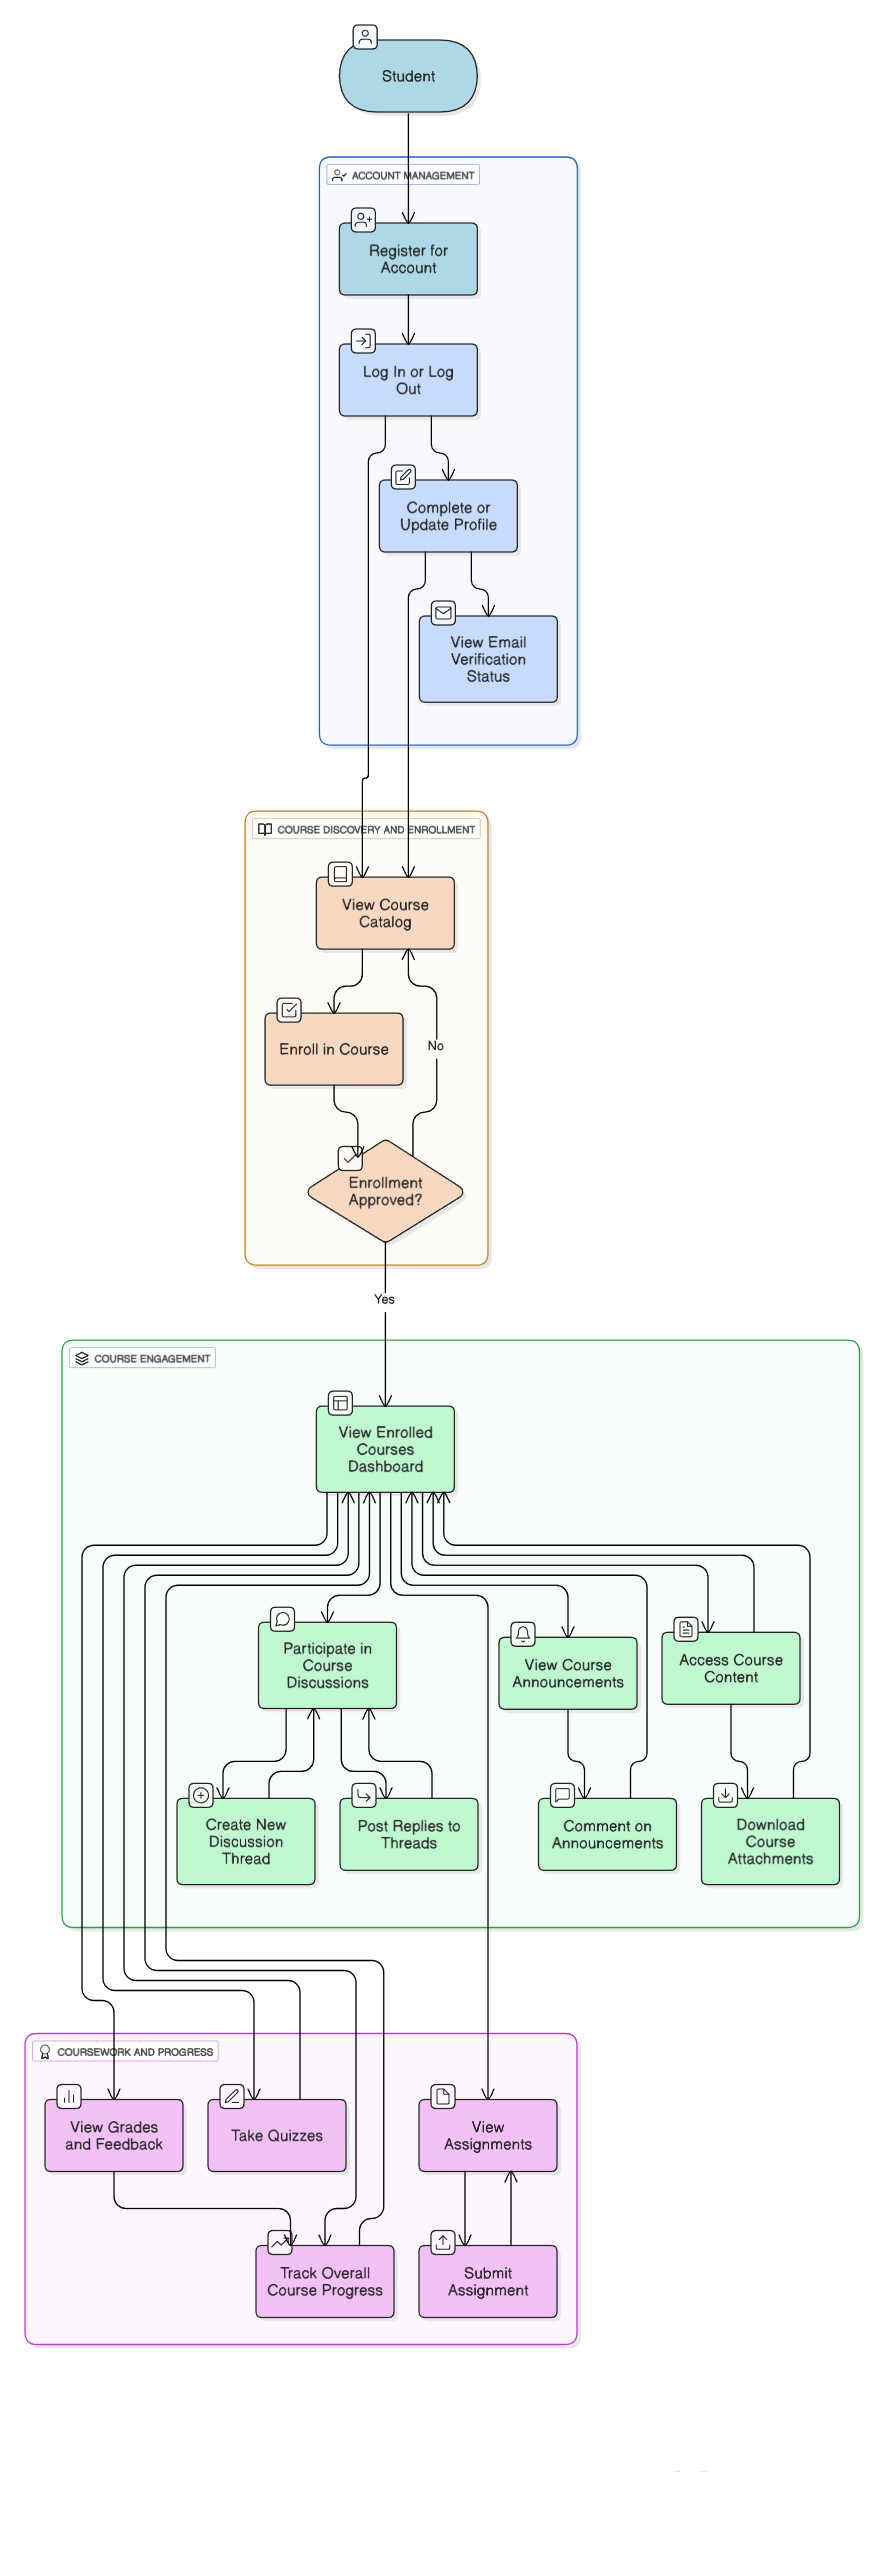
\includegraphics[width=0.8\textwidth,height=0.85\textheight,keepaspectratio]{student-usecase-diagram.png}
        \captionof{figure}{Student Use Case Diagram - showing interactions between students and the learning platform}
        \label{fig:student-usecase}
    \end{center}

    \clearpage
    \item \textbf{Instructor Use Case Diagram}
    
    \begin{figure}[!htbp]
        \centering
        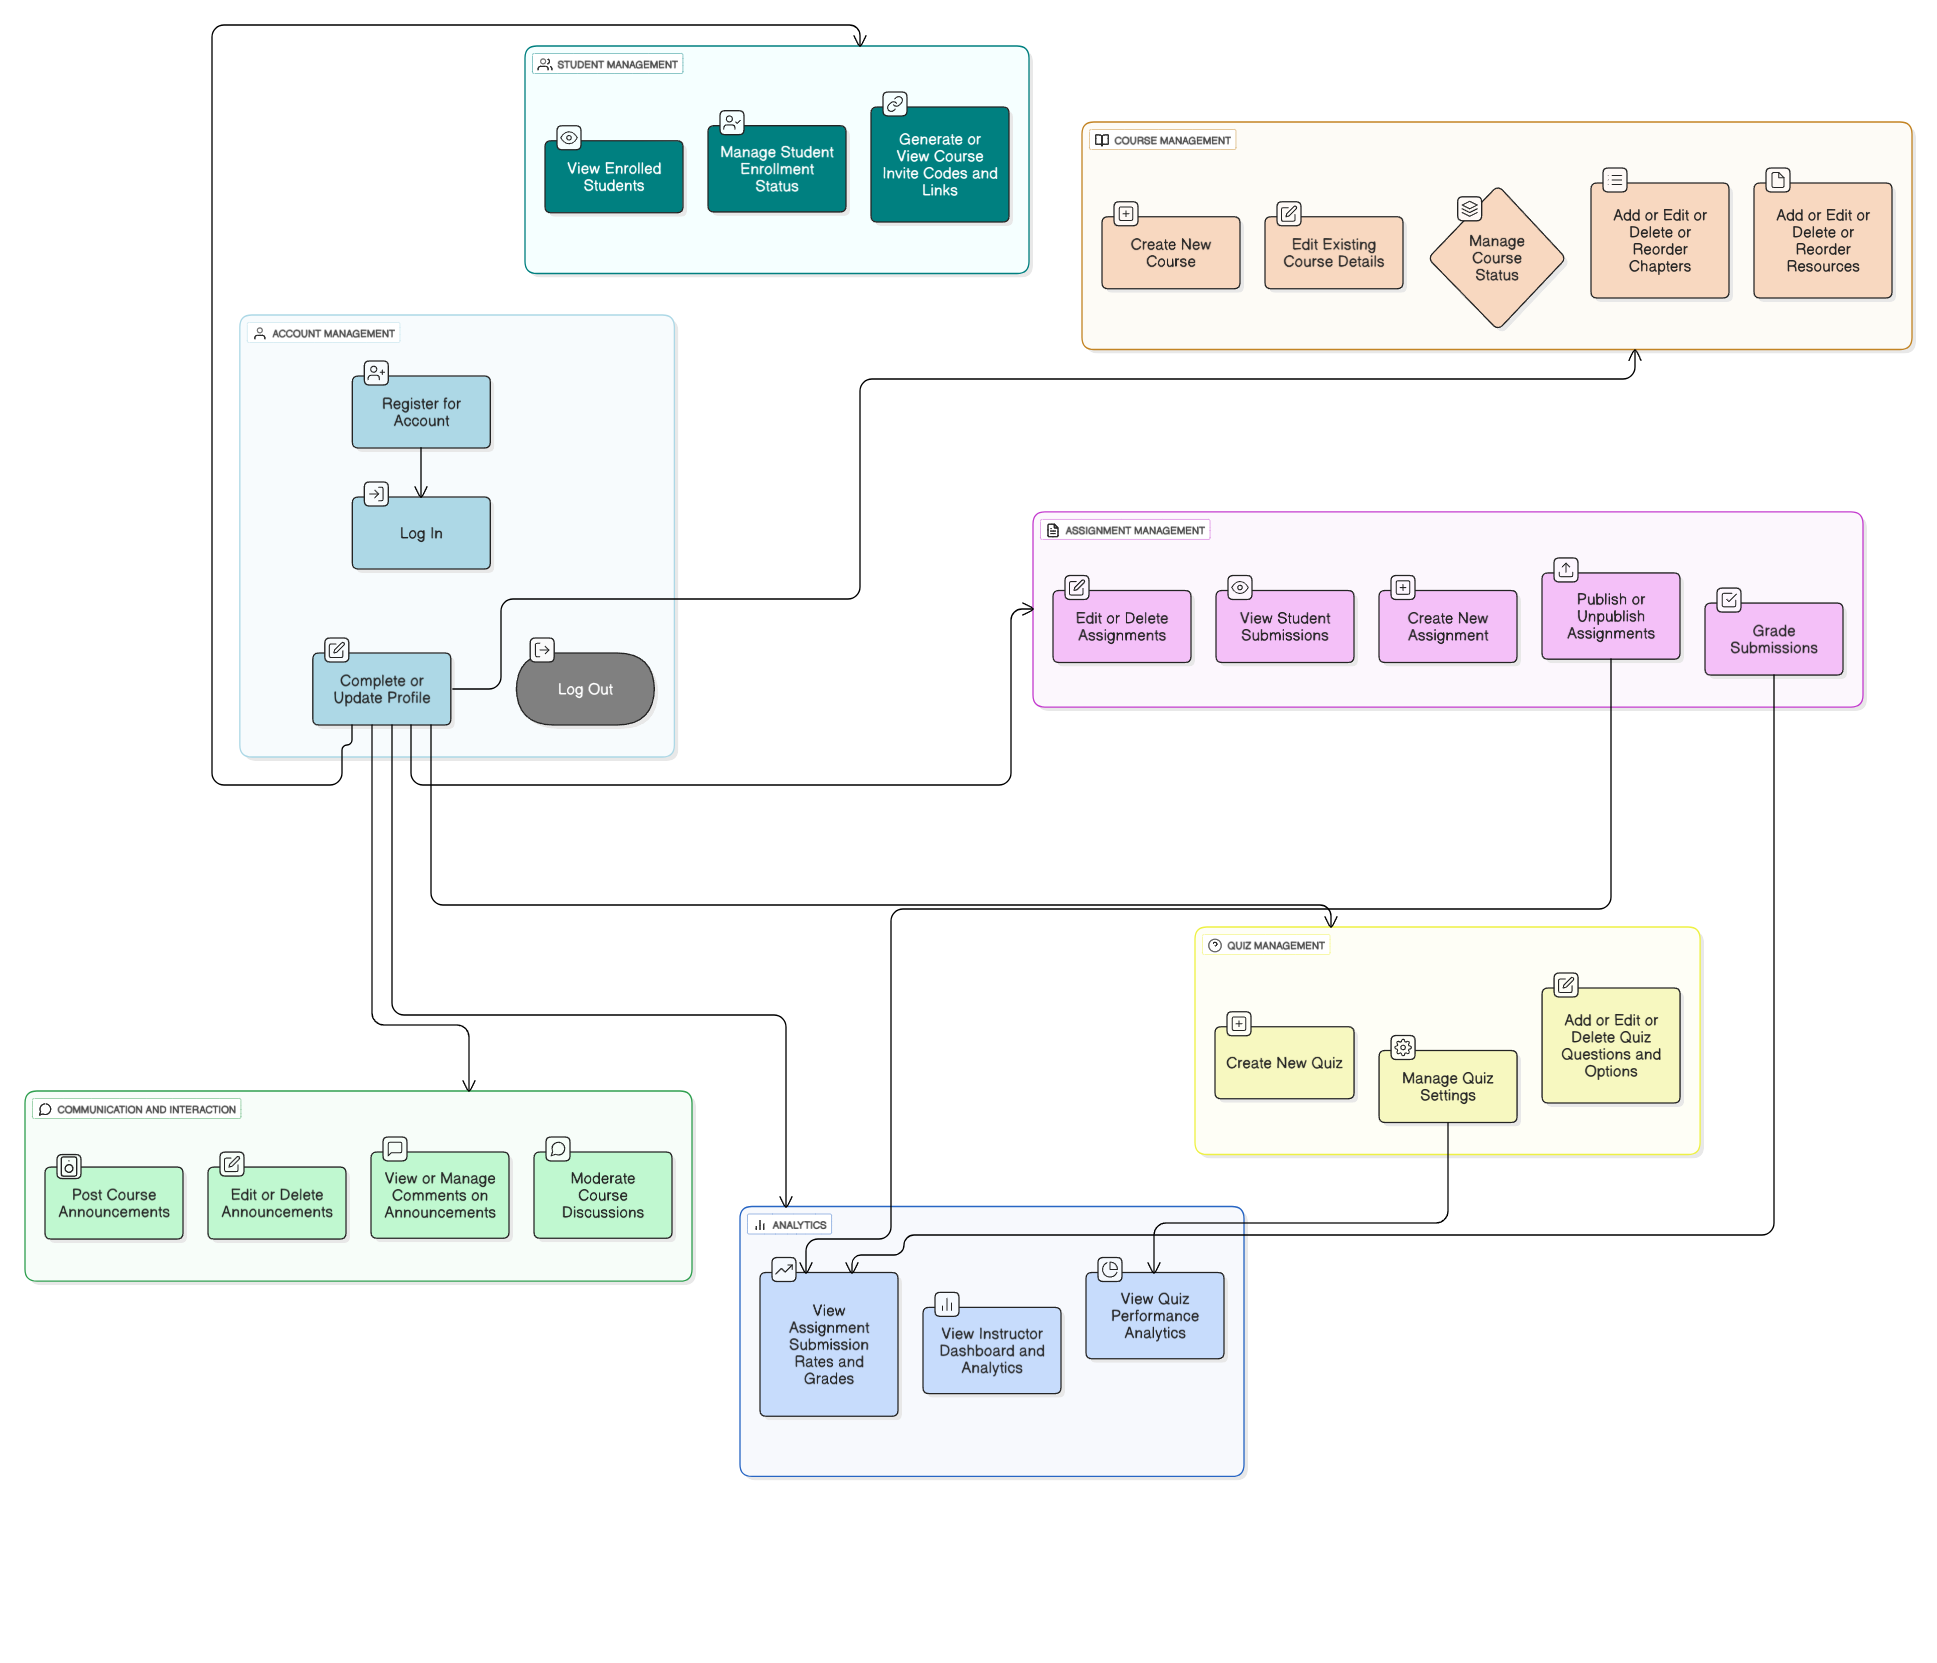
\includegraphics[width=0.9\textwidth]{instructor-usecase-diagram.png}
        \caption{Instructor Use Case Diagram - illustrating instructor functionalities and system interactions}
        \label{fig:instructor-usecase}
    \end{figure}
    \FloatBarrier
    
    \item \textbf{Administrator Use Case Diagram}
    
    \begin{figure}[!htbp]
        \centering
        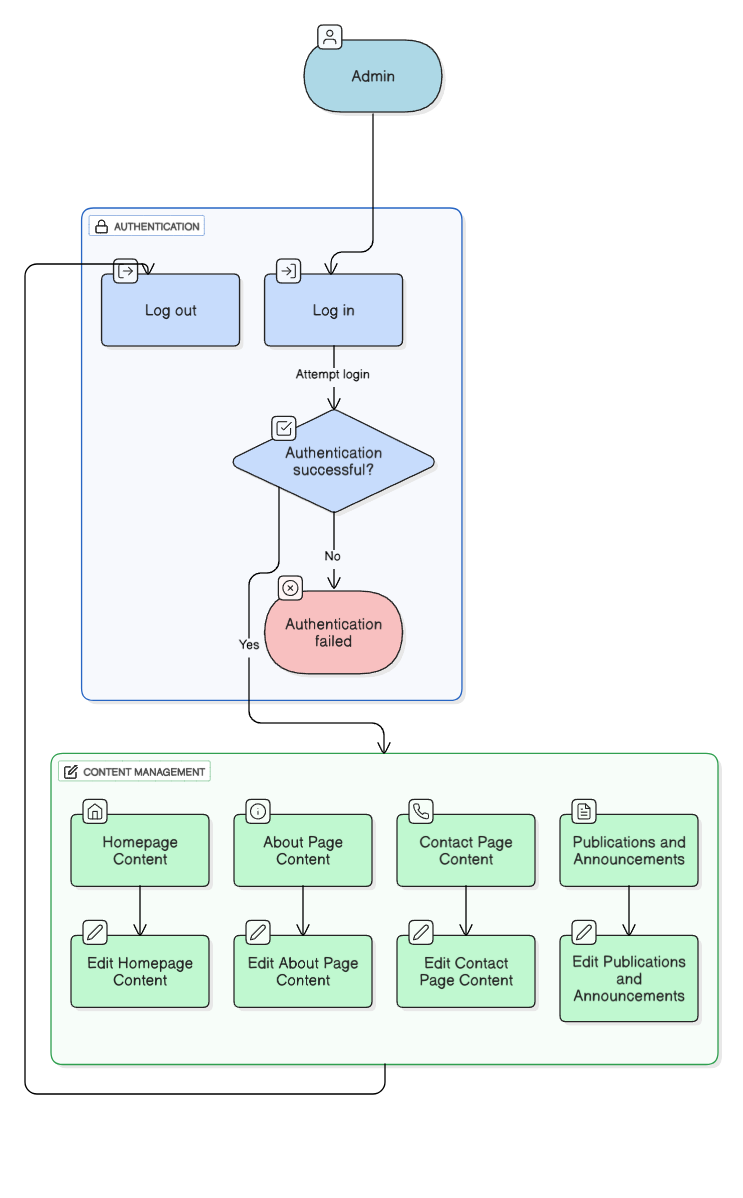
\includegraphics[width=0.9\textwidth]{administrator-usecase-diagram.png}
        \caption{Administrator Use Case Diagram - depicting administrative operations and system management tasks}
        \label{fig:administrator-usecase}
    \end{figure}
    \FloatBarrier
\end{itemize}

\subsection{Sequence Diagrams}

These diagrams trace the flow of information through the system during critical operations, revealing the intricate coordination between frontend, backend, and data storage components:

\begin{itemize}
    \item \textbf{Student Submits Assignment:}
    \begin{center}       
        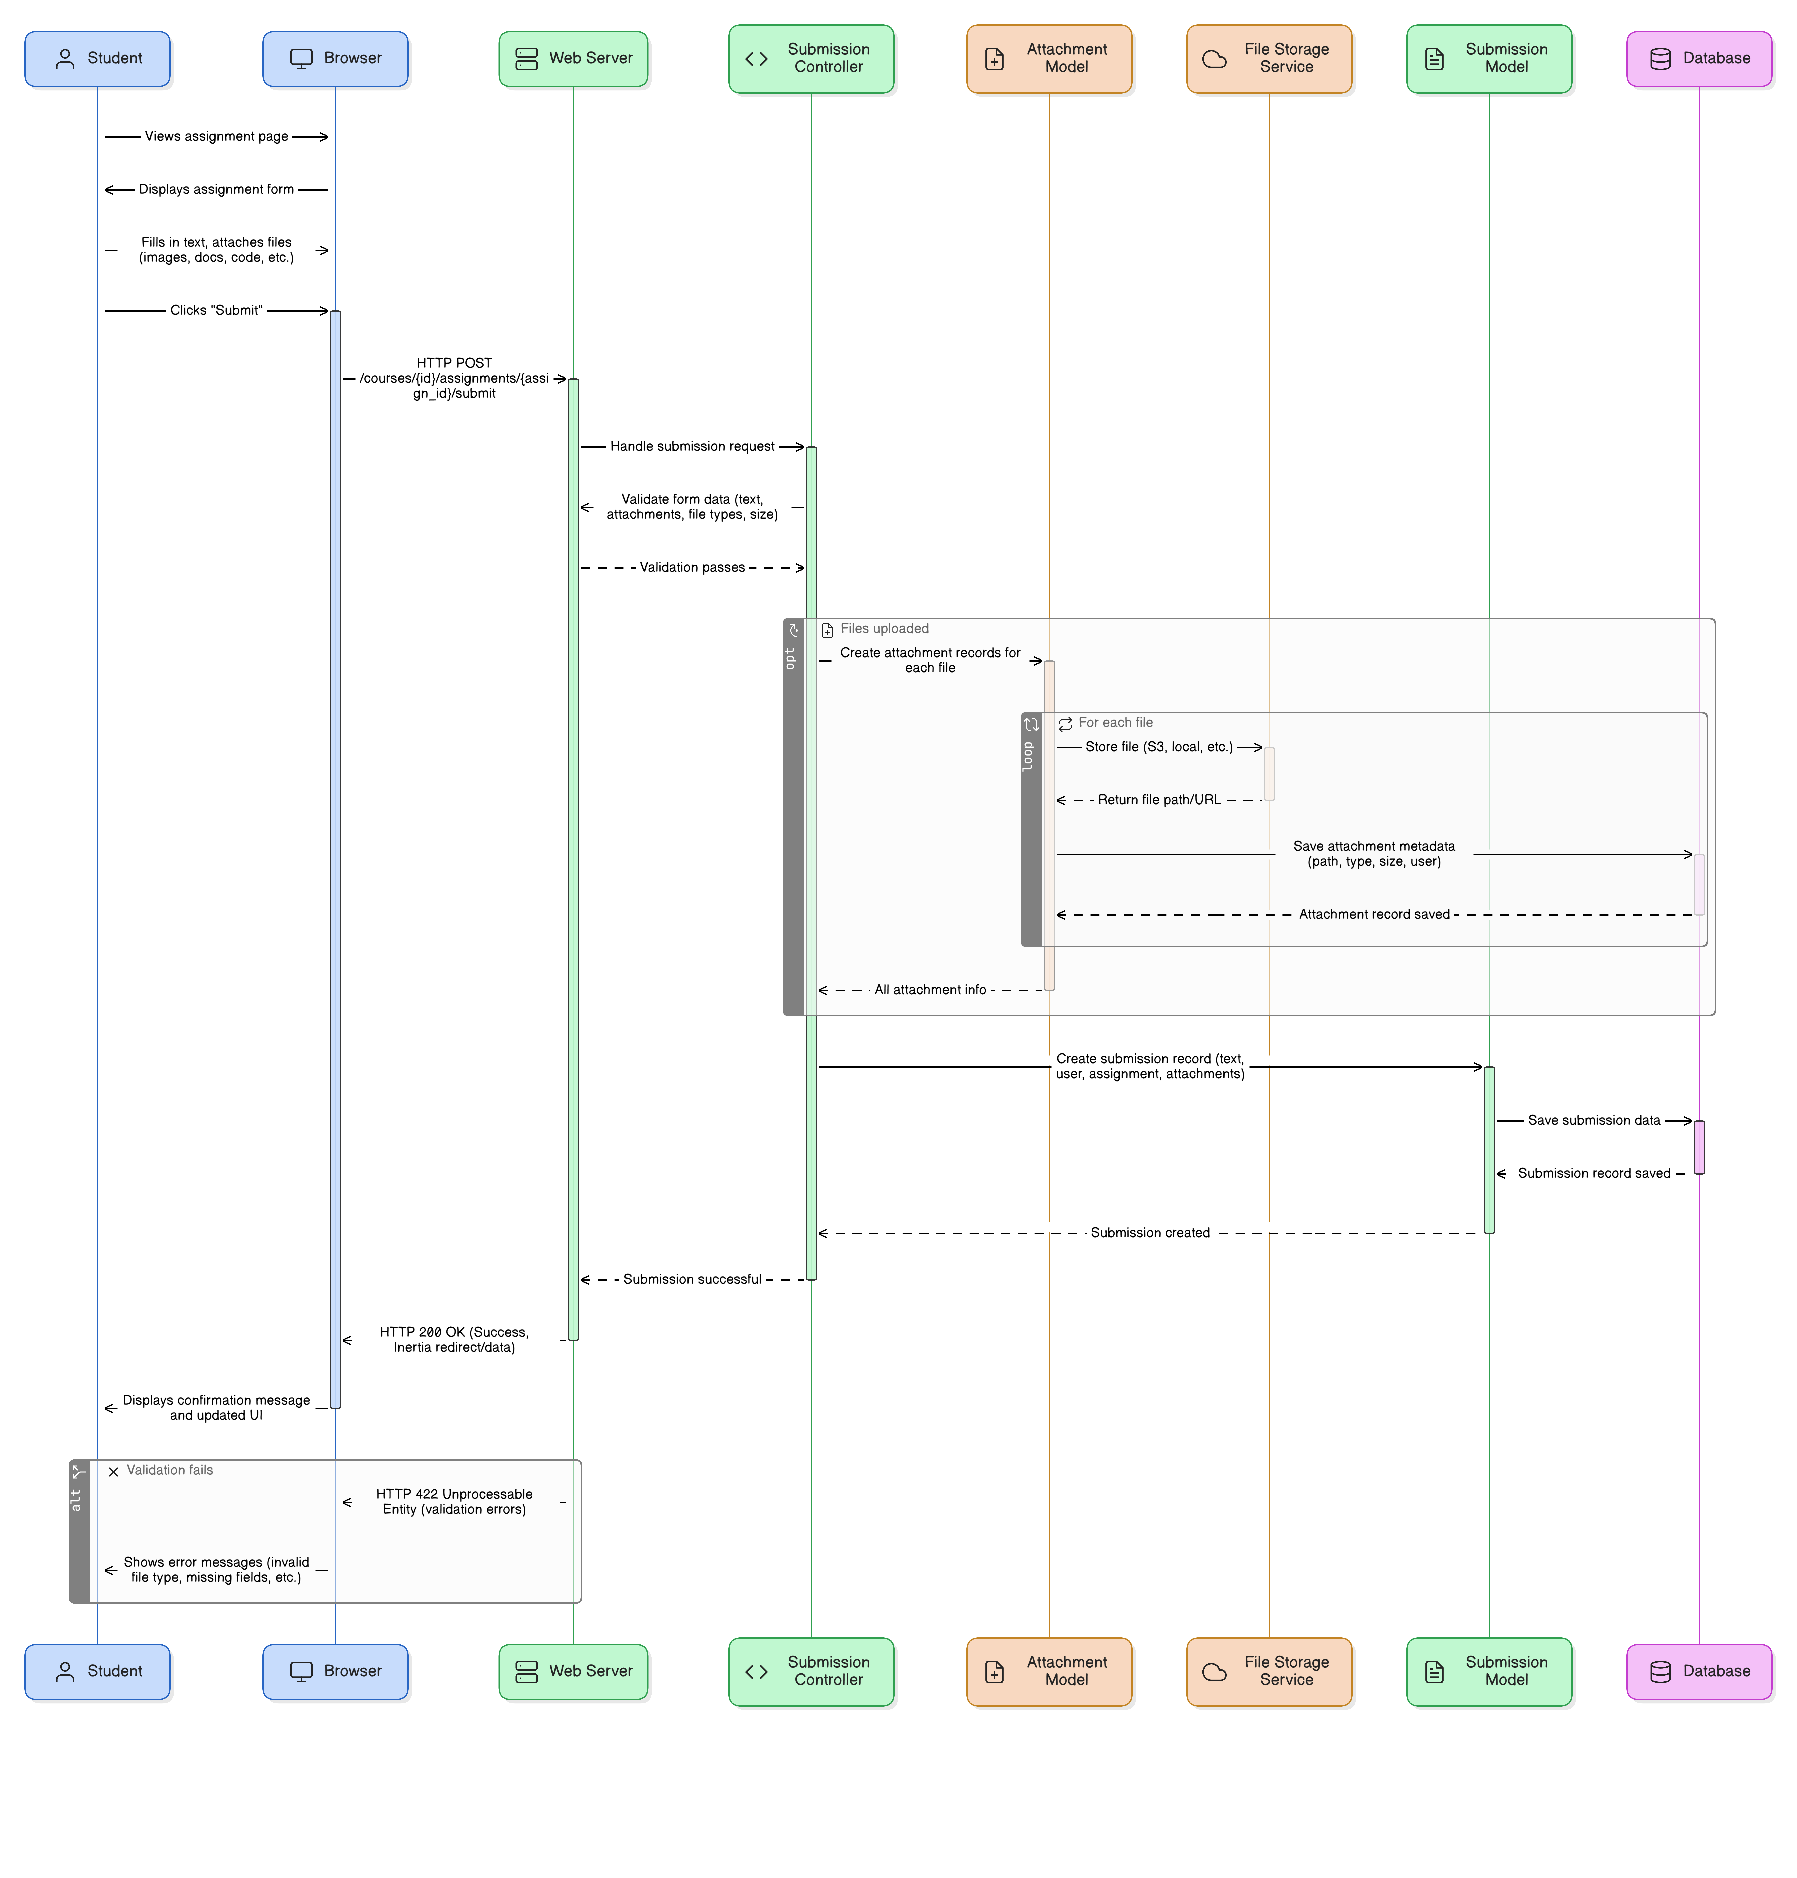
\includegraphics[width=0.8\textwidth,height=0.85\textheight,keepaspectratio]{student-submits-assignment.png}
        \captionof{figure}{Student assignment submission sequence diagram}
        \label{fig:student-submits-assignment}
        \end{center}
    \clearpage
    \item \textbf{Instructor Grades Submission:}
    \begin{center}       
        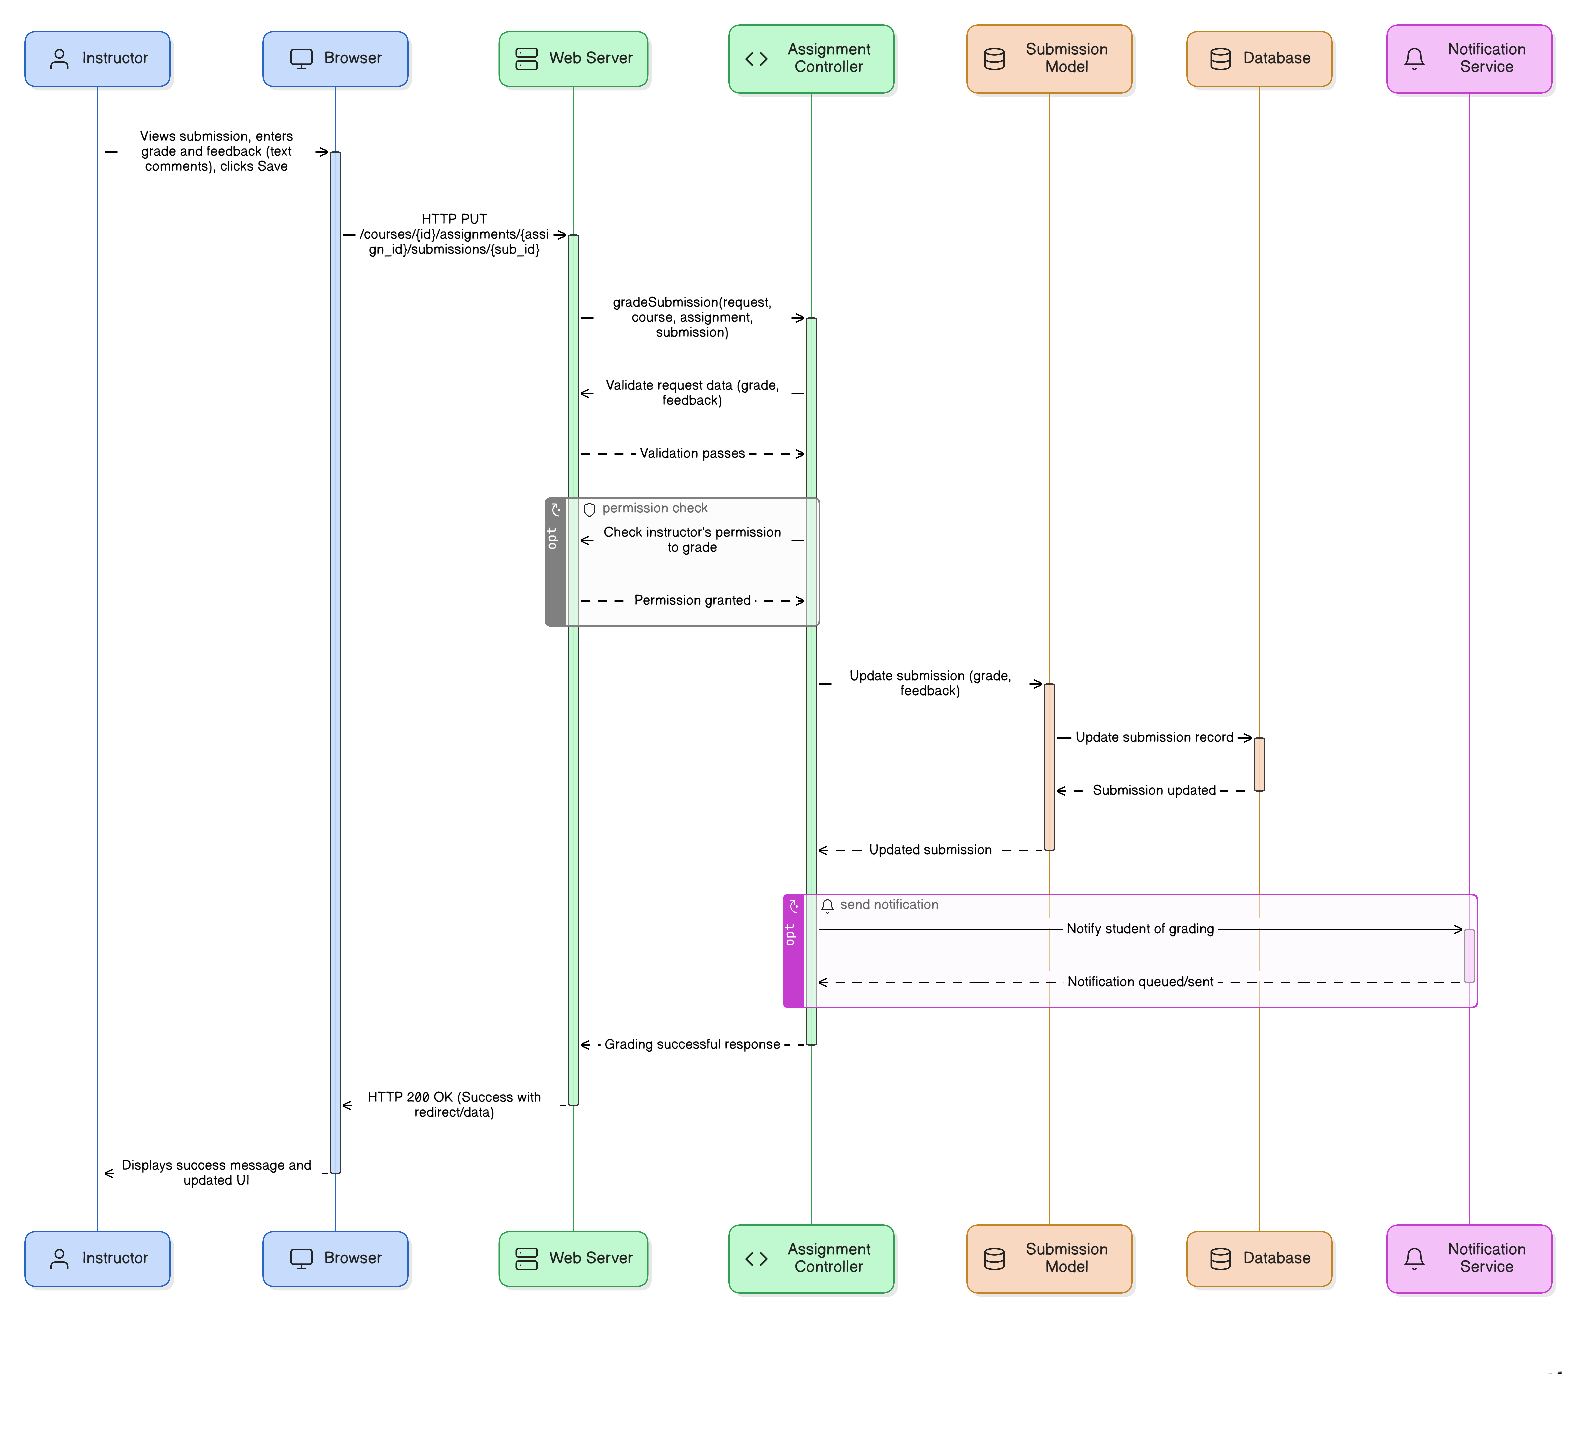
\includegraphics[width=0.8\textwidth,height=0.85\textheight,keepaspectratio]{instructor-grades-submission.png}
        \captionof{figure}{Instructor grading a submission sequence diagram}
        \label{fig:instructor-grades-submission}
        \end{center}
    \clearpage
    \item \textbf{User (Student/Instructor) Authenticates (Login):}
    \begin{center}       
        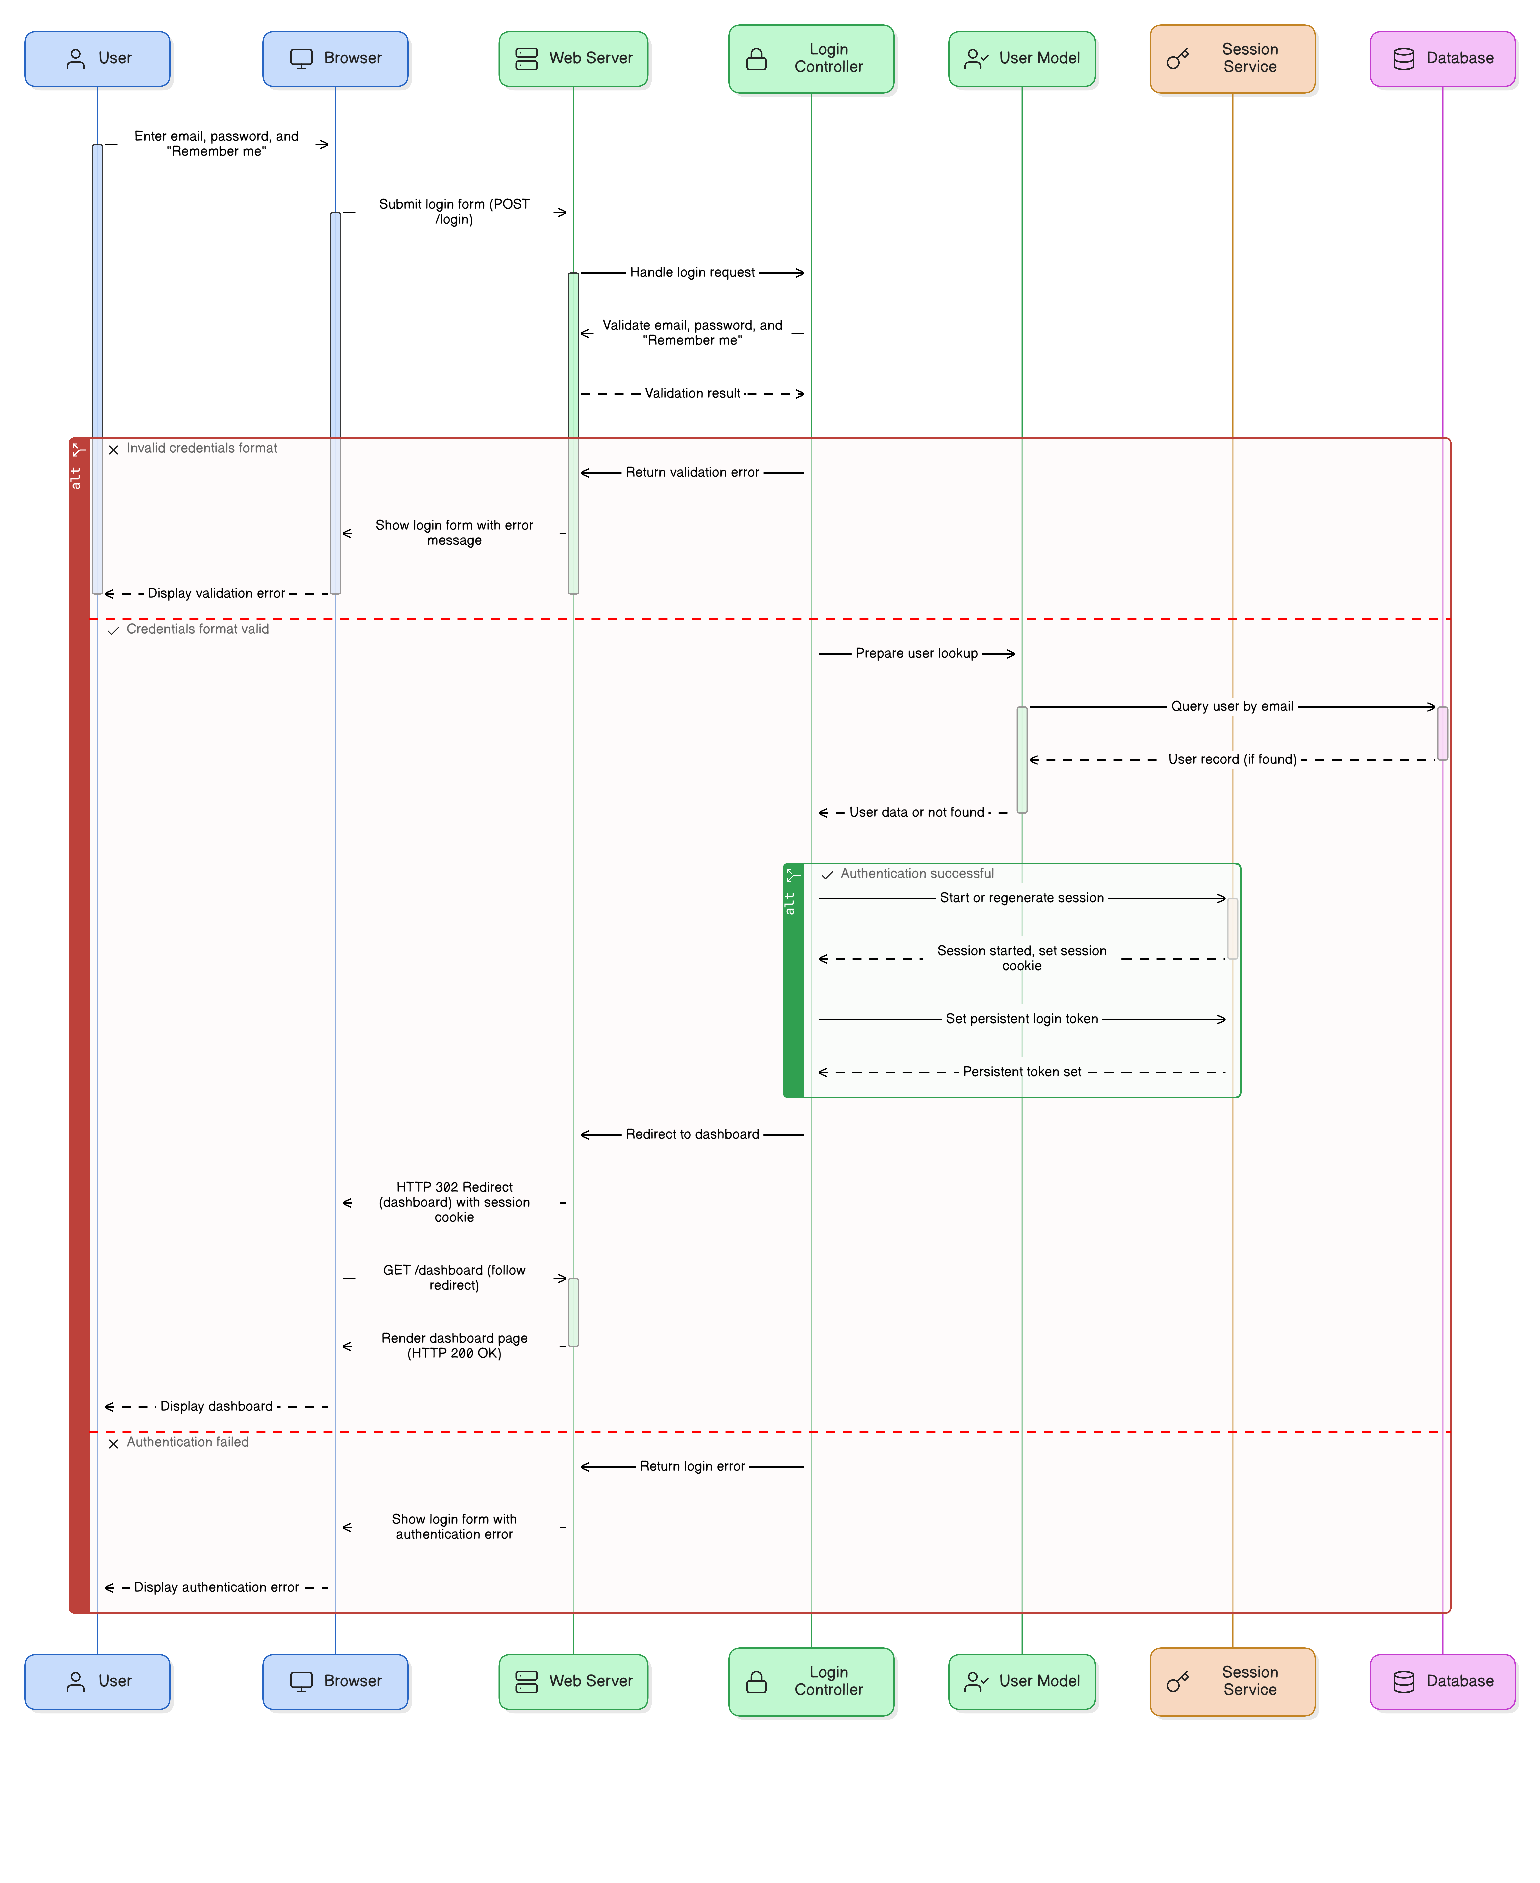
\includegraphics[width=0.8\textwidth,height=0.85\textheight,keepaspectratio]{user-authentication.png}
        \captionof{figure}{User authentication sequence diagram}
        \label{fig:user-authentication}
        \end{center}
        \FloatBarrier
    \clearpage
\end{itemize}

\section{User Interface Design}

\label{sec:ui-design}

The following screenshots provide a comprehensive view of the platform's user interface design and functionality. Each screen demonstrates the practical implementation of the features described in previous sections, showing how users interact with the system across different roles and contexts:

\subsection{Public Pages}
\begin{figure}[H]
    \centering
    \includegraphics[width=\textwidth]{images/ensiasd.elguarir.dev_.png}
    \caption{Platform Homepage - Main landing page with hero section, popular courses, and calls to action.}
    \label{fig:screen-homepage}
\end{figure}
\FloatBarrier

\begin{figure}[H]
    \centering
    \includegraphics[width=\textwidth]{images/ensiasd.elguarir.dev_courses.png}
    \caption{Course Courses Page - Browse, search, and filter available courses.}
    \label{fig:screen-course-listing}
\end{figure}
\FloatBarrier

\begin{figure}[H]
    \centering
    \includegraphics[width=\textwidth]{images/ensiasd.elguarir.dev_publications.png}
    \caption{Course Publications Page - View recent publications.}
    \label{fig:screen-publications}
\end{figure}
\FloatBarrier

\begin{figure}[H]
    \centering
    \includegraphics[width=\textwidth]{images/ensiasd.elguarir.dev_about.png}
    \caption{About Page - Information about ENSIASD and the platform.}
    \label{fig:screen-about}
\end{figure}
\FloatBarrier

\begin{figure}[H]
    \centering
    \includegraphics[width=\textwidth]{images/ensiasd.elguarir.dev_contact.png}
    \caption{Contact Page - ENSIASD contact information and place.}
    \label{fig:screen-contact}
\end{figure}
\FloatBarrier

\begin{figure}[H]
    \centering
    \includegraphics[width=\textwidth]{images/ensiasd.elguarir.dev_login.png}
    \caption{Login Page - Login to the ENSIASD platform.}
    \label{fig:screen-login}
\end{figure}
\FloatBarrier
\clearpage

\subsection{Authenticated User Dashboard \& Internal Pages}

\begin{figure}[H]
    \centering
    \includegraphics[width=\textwidth]{images/ensiasd.elguarir.dev_dashboard.png}
    \caption{Instructor Dashboard - Statistics on courses, students, and quick actions.}
    \label{fig:screen-dashboard-instructor}
\end{figure}
\FloatBarrier

\begin{figure}[H]
    \centering
    \includegraphics[width=\textwidth]{images/ensiasd.elguarir.dev_dashboard (1).png}
    \caption{Course List (Student) - Accessing enrolled courses.}
    \label{fig:screen-course-list-student}
\end{figure}
\FloatBarrier

\begin{figure}[H]
    \centering
    \includegraphics[width=\textwidth]{images/ensiasd.elguarir.dev_dashboard_courses_1.png}
    \caption{Course Content View (Student) - Accessing chapters, resources, assignments, and discussions.}
    \label{fig:screen-course-content-student}
\end{figure}
\FloatBarrier

\begin{figure}[H]
    \centering
    \includegraphics[width=\textwidth]{images/ensiasd.elguarir.dev_login (3).png}
    \caption{Course Join Dialog (Student) - Join a course using a code.}
    \label{fig:screen-course-join}
\end{figure}
\FloatBarrier

\clearpage

\begin{figure}[H]
    \centering
    \includegraphics[width=\textwidth]{images/ensiasd.elguarir.dev_courses_1_threads_1 (2).png}
    \caption{Course Management View (Instructor) - Editing course details, managing chapters and resources.}
    \label{fig:screen-course-management}
\end{figure}
\FloatBarrier

\begin{figure}[H]
    \centering
    \includegraphics[width=\textwidth]{images/ensiasd.elguarir.dev_courses_1_threads_1 (1).png}
    \caption{Course Creation Dialog (Instructor).}
    \label{fig:screen-course-creation}
\end{figure}
\FloatBarrier

\begin{figure}[H]
    \centering
    \includegraphics[width=\textwidth]{images/ensiasd.elguarir.dev_courses_1_threads_1 (4).png}
    \caption{Resources Creation Dialog (Instructor).}
    \label{fig:screen-resource-creation}
\end{figure}
\FloatBarrier

\begin{figure}[H]
    \centering
    \includegraphics[width=\textwidth]{images/ensiasd.elguarir.dev_dashboard_courses_4 (2).png}
    \caption{Resources Creation Dialog (Instructor) - Rich Text Editor.}
    \label{fig:screen-resource-editor}
\end{figure}
\FloatBarrier

\begin{figure}[H]
    \centering
    \includegraphics[width=\textwidth]{images/ensiasd.elguarir.dev_dashboard_courses_4.png}
    \caption{Resources Creation Dialog (Instructor) - Quiz Builder / AI Quiz Generator.}
    \label{fig:screen-resource-quizbuilder}
\end{figure}
\FloatBarrier

\begin{figure}[H]
    \centering
    \includegraphics[width=\textwidth]{images/ensiasd.elguarir.dev_dashboard_courses_1_assignments.png}
    \caption{Assignments View Page (Instructor) - Assignments List.}
    \label{fig:screen-assignment-list}
\end{figure}
\FloatBarrier

\begin{figure}[H]
    \centering
    \includegraphics[width=\textwidth]{images/ensiasd.elguarir.dev_courses_1_assignments_3.png}
    \caption{Assignment Submission Page (Instructor) - Assignment Details.}
    \label{fig:screen-assignment-details}
\end{figure}
\FloatBarrier

\begin{figure}[H]
    \centering
    \includegraphics[width=\textwidth]{images/ensiasd.elguarir.dev_courses_1_assignments_3_submissions.png}
    \caption{Assignment Submissions Page (Instructor) - Assignment Submissions.}
    \label{fig:screen-assignment-submissions}
\end{figure}
\FloatBarrier

\begin{figure}[H]
    \centering
    \includegraphics[width=\textwidth]{images/ensiasd.elguarir.dev_courses_1_assignments_3_submissions (2).png}
    \caption{Grading Interface (Instructor) - Reviewing submissions and providing feedback/grades.}
    \label{fig:screen-grading}
\end{figure}

\FloatBarrier
\clearpage

% \subsection{Administrator Content Management}
% \begin{figure}[H]
%     \centering
%     \framebox(300,200){Placeholder: Screenshot of Admin - Edit Homepage Content} % \includegraphics{path/to/admin_edit_home_screenshot.png}
%     \caption{Administrator View - Editing public homepage content.}
%     \label{fig:screen-admin-edit-home}
% \end{figure}
% \FloatBarrier
% \clearpage

\section{Future Development and Enhancement Opportunities}
\label{sec:future-development}

The current platform establishes a solid foundation for digital education at ENSIASD Taroudant. However, the rapidly evolving landscape of educational technology presents numerous opportunities for expansion and improvement. This section explores potential enhancements that could further strengthen the platform's capabilities and impact:
\subsection{Suggestions for Platform Enhancements}
\begin{enumerate}
    \item \textbf{Advanced Analytics \& Reporting:}
    \begin{itemize}
        \item \textit{For Students:} More detailed personal progress dashboards.
        \item \textit{For Instructors:} Deeper insights into student engagement, assignment difficulty, and at-risk student indicators.
        \item \textit{For Administrators:} Comprehensive platform usage reports.
    \end{itemize}
    \item \textbf{Mobile Application:}
    \begin{itemize}
        \item Develop native or hybrid mobile apps for on-the-go access, offline content, and push notifications.
    \end{itemize}
    \item \textbf{Integrations with External Services:}
    \begin{itemize}
        \item \textbf{Live Virtual Classes:} Integration with tools like Zoom or BigBlueButton.
        \item \textbf{Calendar Integration:} Syncing deadlines with Google/Outlook Calendar.
        \item \textbf{Plagiarism Detection:} Tools like Turnitin.
        \item \textbf{Single Sign-On (SSO):} Integration with institutional identity providers.
    \end{itemize}
    \item \textbf{Enhanced Accessibility (a11y):}
    \begin{itemize}
        \item Continuous audits and improvements based on WCAG guidelines to ensure inclusivity.
    \end{itemize}
    \item \textbf{Personalized Learning Paths \& AI Features:}
    \begin{itemize}
        \item Adaptive learning paths based on student performance.
        \item AI-powered recommendations or support bots.
    \end{itemize}
    \item \textbf{Improved Search Functionality:}
    \begin{itemize}
        \item Global search across all enrolled courses and content types.
    \end{itemize}
    \item \textbf{Interactive Content Types:}
    \begin{itemize}
        \item Support for H5P or SCORM packages for richer interactive content.
    \end{itemize}
\end{enumerate}

\subsection{Platform Development and Operational Considerations}
\begin{enumerate}
    \item \textbf{Deployment Strategy \& Infrastructure:}
    \begin{itemize}
        \item Standard LEMP/LAMP stack deployment. Key steps include code deployment, dependency installation, configuration, migrations, queue worker setup, and task scheduling.
        \item Automation tools (Forge, Ploi, CI/CD pipelines) can simplify this.
    \end{itemize}
    \item \textbf{Security Considerations:}
    \begin{itemize}
        \item Leverage Laravel's built-in features (CSRF, XSS, SQLi prevention, hashing).
        \item Application-level measures: input validation, RBAC, HTTPS.
        \item Ongoing practices: dependency updates, audits, secure file handling, rate limiting.
    \end{itemize}
    \item \textbf{Scalability Aspects:}
    \begin{itemize}
        \item Horizontal scaling of application servers.
        \item Database scaling (read replicas, cloud solutions).
        \item Extensive caching (Redis).
        \item Background jobs for time-consuming tasks.
        \item CDN for static assets.
    \end{itemize}
    \item \textbf{Project Management Methodology (Suggested):}
    \begin{itemize}
        \item Agile methodologies (Scrum, Kanban) are well-suited for iterative development and stakeholder feedback.
    \end{itemize}
    % Contribution Guidelines can be omitted if not directly relevant to the report's current scope
\end{enumerate}
\clearpage


\section{Conclusion}
\label{sec:conclusion}

The ENSIASD E-Learning Platform stands as a testament to thoughtful educational technology design, successfully bridging the gap between traditional academic instruction and modern digital learning requirements. Through its sophisticated integration of Laravel's robust backend capabilities with React's dynamic frontend experience, the platform creates an environment where education technology serves pedagogical goals rather than constraining them.

The platform's architecture demonstrates careful consideration of the diverse stakeholder needs within higher education. Students benefit from intuitive interfaces that prioritize learning over navigation complexity, while instructors gain powerful content creation and assessment tools that enhance rather than complicate their teaching workflows. Administrators receive comprehensive oversight capabilities that maintain institutional standards while supporting academic freedom.

Perhaps most significantly, the platform's technical foundation positions ENSIASD Taroudant for continued innovation in digital education. The modular architecture, contemporary technology stack, and extensible design patterns create numerous opportunities for enhancement and adaptation as educational needs evolve.

This analysis reveals not just a functional e-learning system, but a platform designed for growth, adaptation, and sustained educational impact. The careful balance between current functionality and future flexibility suggests that ENSIASD Taroudant has invested in technology that will continue serving its educational mission for years to come.

\end{document}